\documentclass[12p,a4paper]{report}
\usepackage[english]{babel}
\usepackage[utf8]{inputenc}
\usepackage{graphicx}
\graphicspath{{Figures/}}
\usepackage[top=25mm,bottom=25mm]{geometry}

\usepackage[style=alphabetic]{biblatex}
\addbibresource{references.bib}

\title{
    {\large Luleå University of Technology (LTU)}\\
    {\large Department of Computer Science, Electrical and Space Engineering}\\
    {\large Digital Services and Systems}\\
    {\large COURSE: D0025E}\\
    {Data Mining Assignment Number 1: CORRELATIONS}\\
    {\centering
\includegraphics{LTUlogo.png}}\\
}

\author{GROUP NO.: x, MEMBERS: a,b,c,d,e}
\date{LP1-2025}

\begin{document}

\maketitle

\chapter*{Abstract}
This is the summary of the document ...


\chapter*{Highlights}
This is the assignment highlights on which we would like to highlight the following points that we think are key:
\begin{itemize}
    \item Theory 
\title{
    {The CRISP-DM Process}\\
    {\centering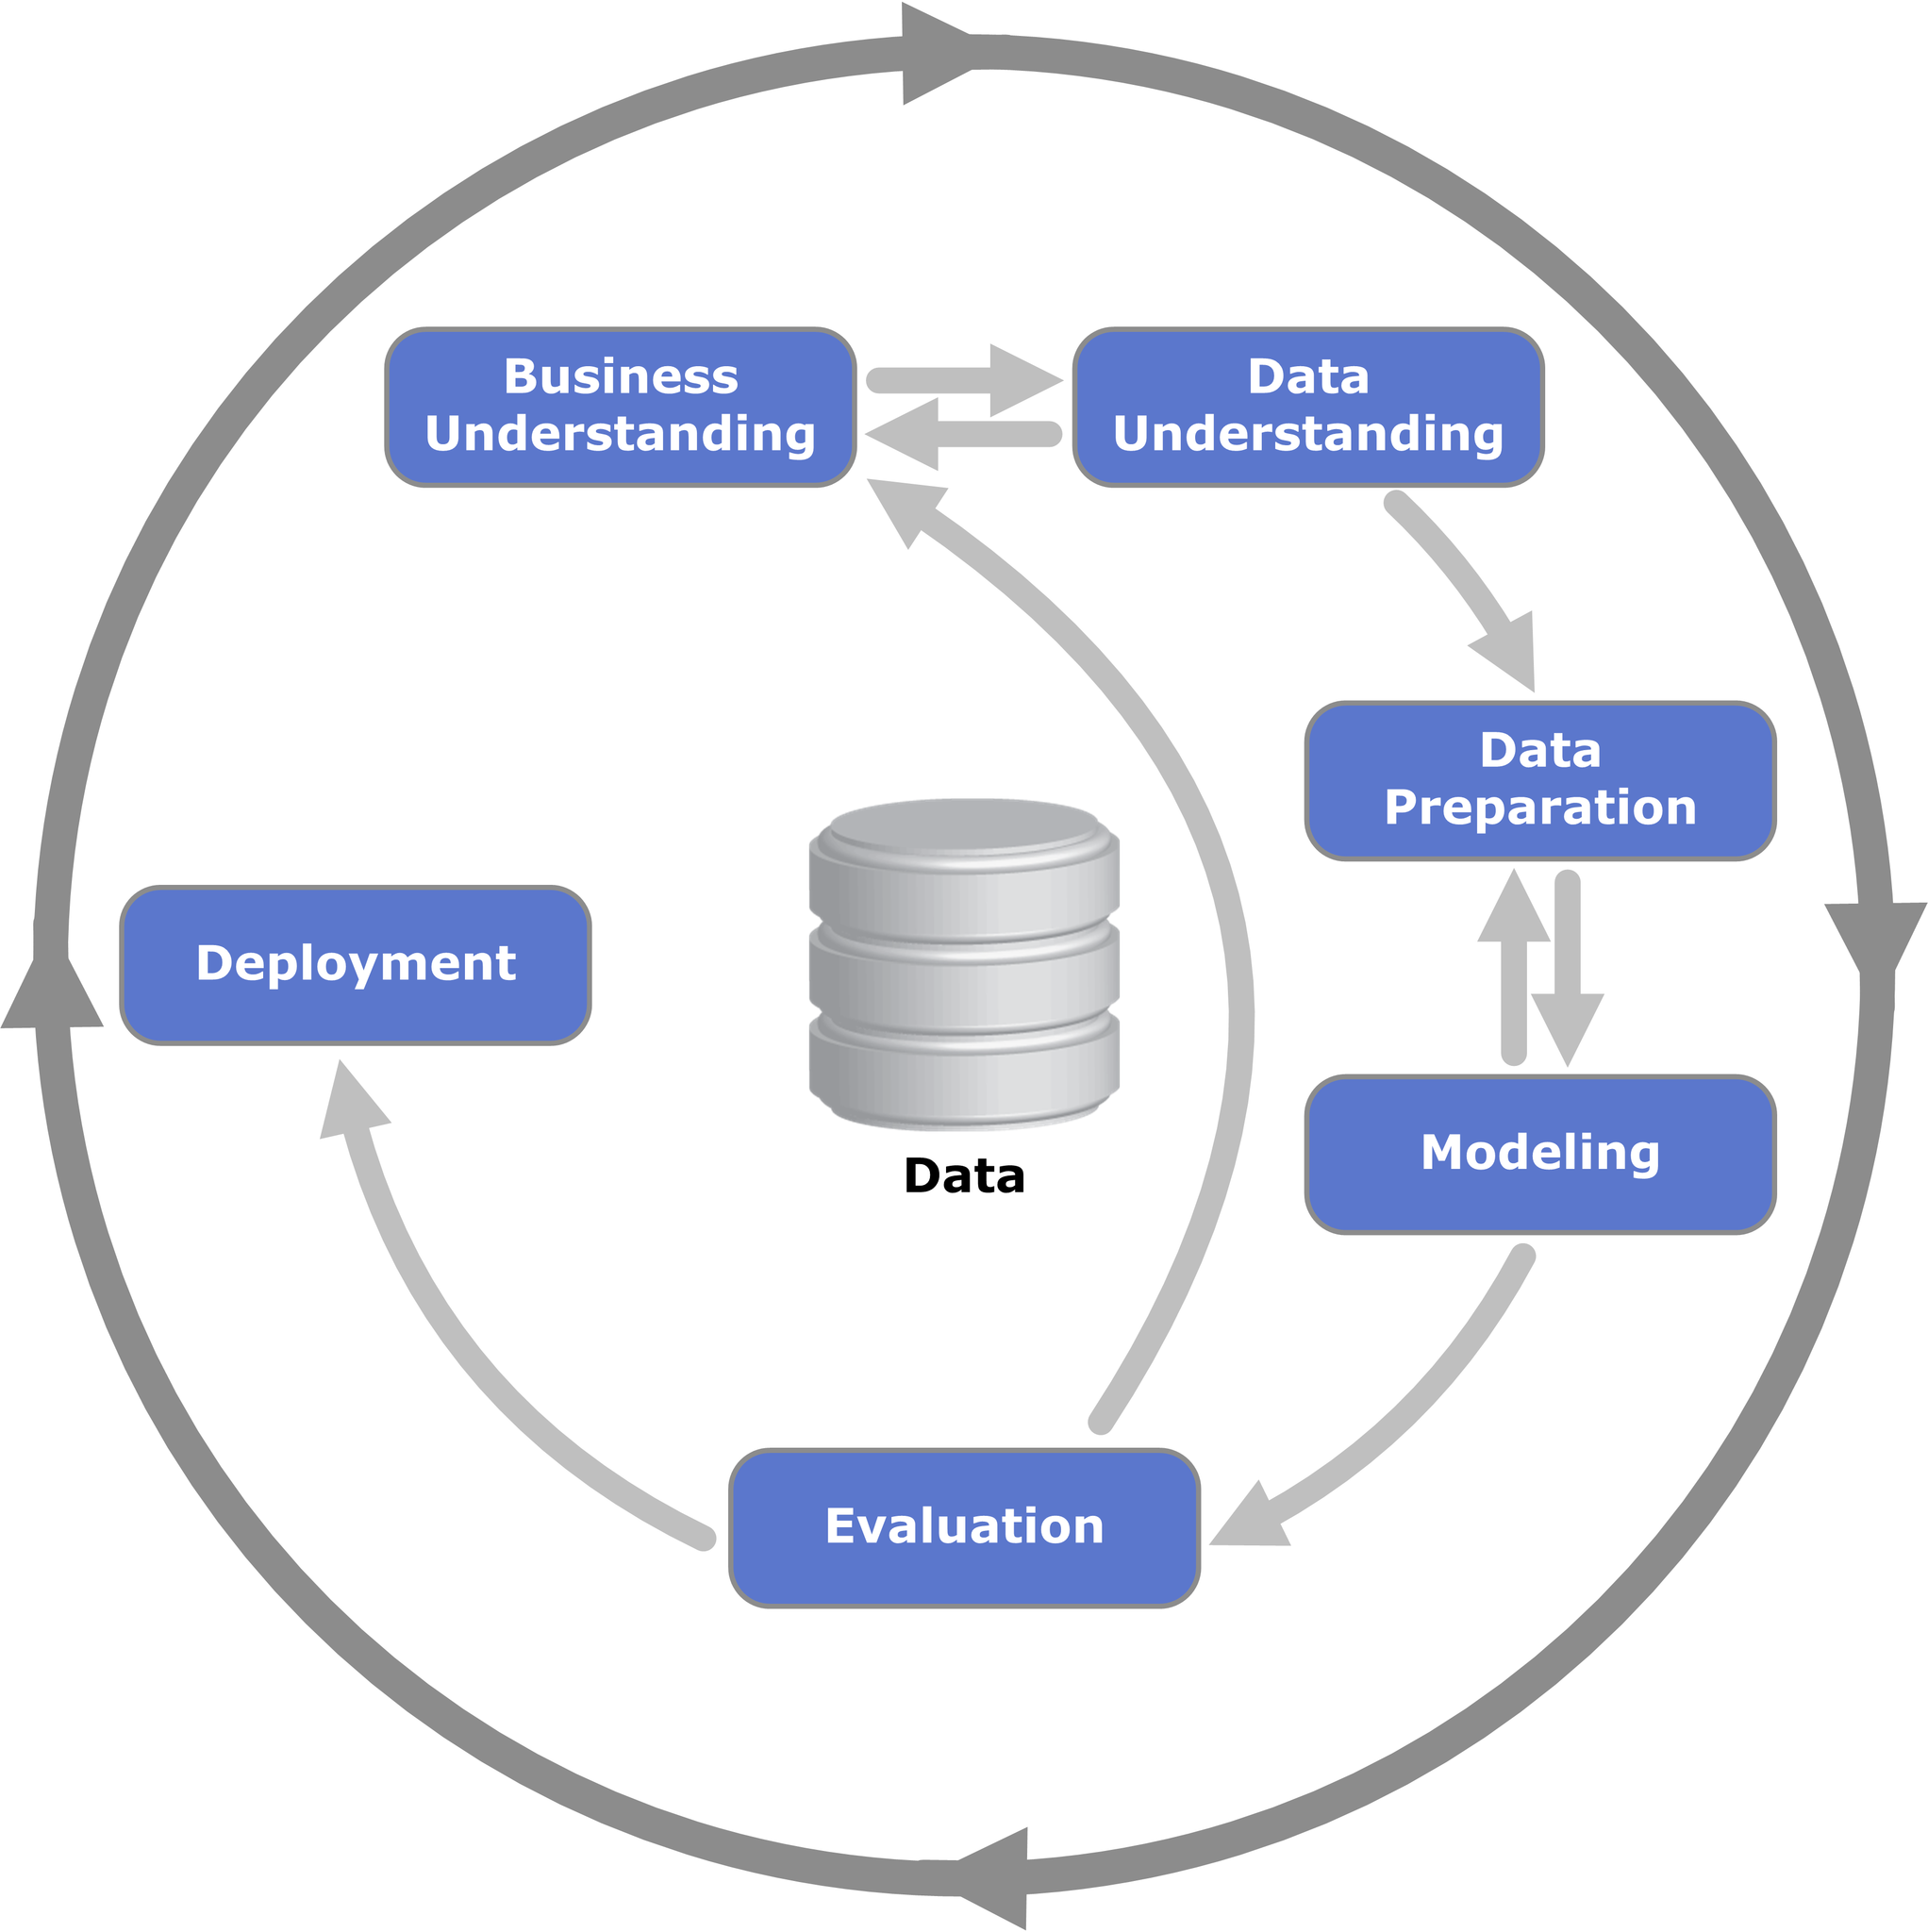
\includegraphics{Figures/crispdm2.png}}\\
}
    \item Practice
    \item Others
\end{itemize}

\tableofcontents

\chapter{Phase I: Business Understanding}
The Business Understanding Phase:

This chapter is a \emph{key}!

\begin{enumerate}
  \item This is the first entry in my list
  \item This is the second entry in my list
  \item This is the third entry in my list
\end{enumerate}

\begin{center}
    \begin{tabular}{ c c c }
        cell1 & cell2 & cell3 \\ 
        cell4 & cell5 & cell6 \\  
        cell7 & cell8 & cell9    
    \end{tabular}
\end{center}

\begin{center}
    \begin{tabular}{ |c| c| c| }
     \hline
        cell1 & cell2 & cell3 \\ 
        cell4 & cell5 & cell6 \\  
        cell7 & cell8 & cell9 \\  
     \hline
    \end{tabular}\\
    \caption{Insert Table Caption here!}
    \label{table:1}
\end{center}

\chapter{Phase II: Data Understanding}
The Data Understanding Phase:

'text in single quotation'

''text in double quotations''\\

One of today’s key technologies is \textbf{Big Data}\\
One of today’s key technologies is \textit{Big Data}\\
One of today’s key technologies is \underline{Big Data}\\

Here I am referring to the source \cite{BigData}.

\chapter{Phase III: Data Preprocessing}
The Data Preprocessing Phase:

\begin{equation}
\alpha + \beta + 1
\end{equation}

In this section, we try to use the footnote feature. Test \footnote{Insert whatever content you want e.g., URL} the text when adding the footnote.

Here I am referring to the source \cite{DataScience}.

\chapter{Phase IV: Modeling}
The Modeling Phase:

\$\%\&\#!

\chapter{Phase V: Evaluation}
The Evaluation Phase:

% see how to write a mathematical formula below (note: this line is marked as comment!)
Let $a$ and $b$ be distinct positive integers, and let $c = a - b + 1$

$\mu = a + b $


$\Omega = a - b $

$y = c_2 x^2 + c_1 x + c_0 $

The roots of a quadratic equation are given by:

\begin{equation}
x = \frac{-b \pm \sqrt{b^2 - 4ac}} {2a}
\end{equation}

where $a$, $b$ and $c$ are \ldots


\chapter{Phase VI: Deployment}
The Deployment Phase:



\chapter{Tools Insights}
Tools Insights:



\section{RapidMiner Insights}
This section explains your insights while using RapidMiner to solve assignment number 1 in the course. 

\subsection{Ease of Use 1: ...}
    
\subsection{Efficiency 2: ...}
    
\subsection{Costs 3: ...}

\section{Knime Insights}
This section explains your insights while using Knime to solve assignment number 1 in the course. 

\subsection{Ease of Use 1: ...}
    
\subsection{Efficiency 2: ...}
    
\subsection{Costs 3: ...}

\chapter{Answers to Assignment Questions}
Answers to Assignment Questions:



\section{Question 1 ...}
In this section, you answer the questions associated with the assignment. Question one ...

\section{Question 2 ...}
In this section, you answer the questions associated with the assignment. Question two ...

\section{Question 3 ...}
In this section, you answer the questions associated with the assignment. Question three ...

\chapter{Conclusion}
In this assignment we have done ... We have learned ... We recommend ...

\printbibliography

\end{document}
